\documentclass[russian]{article}
\usepackage[T1]{fontenc}
\usepackage[utf8]{inputenc}
\usepackage{geometry}
\geometry{verbose,tmargin=2cm,bmargin=2cm,lmargin=1cm,rmargin=1cm}
\usepackage{amsmath}
\usepackage{float}
\usepackage{tikz}
\usetikzlibrary{automata,positioning}
\usepackage{textcomp}
\usepackage{amssymb}
\usepackage{graphicx}
\usepackage{babel}
\usepackage{mathtools}
\usepackage{color}
\usepackage[T2A]{fontenc}
\makeatletter
\@ifundefined{date}{}{\date{}}
\begin{document}

\title{Формальные грамматики. HW\#2}
\author{Тураев Тимур, SPbAU, SE, 6$\varnothing$4 group}
\maketitle

\paragraph*{1.}

\textit{Постоить обыкновенную грамматику в нормальном виде Хомского для языка Дика $D=\{\varepsilon, ab, aabb, abab, aaabbb, \ldots\}$ над алфавитом $\{a,b\}$. Для этой грамматики и для входной строки $w=abaabba \notin D$, построить таблицу разбора $T_{i,j}$, как в алгоритме Кокка–Касами–Янгера.}

Обыкновенная грамматика не в нормальной форме:
\begin{align*}
S \to aSb \mid SS \mid \varepsilon
\end{align*}

Приведем эту грамматику к нормальной форме Хомского:

\begin{itemize}
\item Удалим длинное правило $S \to aSb$
\begin{align*}
S & \to Tb \mid SS \mid \varepsilon \\
T & \to aS
\end{align*}

\item Удалим $\varepsilon$-правила:
\begin{align*}
S & \to C \mid \varepsilon \\
C & \to Tb \mid CC \\
T & \to a \mid aC
\end{align*}

\item Удалим цепные правила:
\begin{align*}
S & \to Tb \mid CC \mid \varepsilon \\
C & \to Tb \mid CC \\
T & \to a \mid aC
\end{align*}

\item Последний шаг: заменим терминалы на нетерминалы (бесполезных символов в грамматике нет):
\begin{align*}
S & \to TB \mid CC \mid \varepsilon \\
C & \to TB \mid CC \\
T & \to a \mid AC \\
A & \to a \\
B & \to b
\end{align*}
\end{itemize}

Таблица разбора в алгоритме Кокка–Касами–Янгера:

\begin{align*}
\begin{tabular}{c | c c c c c c c}
	~ & a & b & a & a & b & b & a \\
	\hline
	a & \{A, T\} & \{S, C\} & $\varnothing$ & $\varnothing$ & $\varnothing$ & \{S, C\} & $\varnothing$  \\
	b & ~ & \{B\} & $\varnothing$ & $\varnothing$ & $\varnothing$ & $\varnothing$ & $\varnothing$  \\
	a & ~ & ~ & \{A, T\} & $\varnothing$ & \{T\} &  \{S, C\} & $\varnothing$ \\
	a & ~ & ~ & ~ & \{A, T\} &  \{S, C\} & $\varnothing$ & $\varnothing$  \\
	b & ~ & ~ & ~ & ~ & \{B\} & $\varnothing$ & $\varnothing$  \\
	b & ~ & ~ & ~ & ~ & ~ & \{B\} & $\varnothing$  \\
	a & ~ & ~ & ~ & ~ & ~ & ~ & \{A, T\}  \\
\end{tabular}
\end{align*}

По значению отсутствию нетерминала $S$ в $T_{0, 7}$ видно что да, данная строка не принадлежит языку.

\pagebreak

\paragraph*{2.}

\textit{Рассмотреть работу алгоритма Валианта для грамматики, построенной в прошлом упражнении. Среди всех действий, производимых алгоритмом, найти то произведение булевых матриц, после вычисления которого станет верным условие $S \in f(P_{0,6})$, где $S$ — начальный символ грамматики. Описать, когда и как именно вычисляется это произведение — то есть, какая процедура, вызванная с какими значениями, и какой оператор в ней умножает какие две булевы матрицы какого размера, каков результат умножения, и какие элементы $P_{i,j}$ будут этим затронуты?}

\paragraph*{3.}

\textit{Замкнут ли класс LL языков относительно пересечения с регулярными языками? Если замкнут, привести построение, а если незамкнут, привести пример LL грамматики и регулярного языка с доказательством несуществования LL грамматики для их пересечения}

Рассмотрим такой язык $L_1$ (он задает все строки четной длины, первая половина которых состоит только из букв a, а вторая -- из любых сочетаний букв b и c):

\begin{align*}
L_1 = \{ a^n(b|c)^n \mid n \geqslant 0 \}
\end{align*}

Это $LL(1)$-язык, для него можно построить такую грамматику:

\begin{align*}
S & \to aSB \mid \varepsilon \\
B & \to b \mid c 
\end{align*}

и следующую таблицу разбора:

\begin{align*}
\begin{tabular}{c | c c c c |}
	~ & a & b & c & $\varepsilon$ \\
	\hline
	S & S $\to$ aSB & S $\to$ $\varepsilon$ & S $\to$ $\varepsilon$ & S $\to$ $\varepsilon$ \\
	B & -- & B $\to$ b & B $\to$ c& B $\to$ $\varepsilon$ \\
	\hline
\end{tabular}
\end{align*}

Наряду с $L_1$ рассмотрим язык $L_2$, задающий все слова, в котором сначала идет какое-то (возможно нулевое) число букв a, а затем какое-то (возможно нулевое) число букв b:

\begin{align*}
L_2 = \{ a^nb^m + a^nc^m\mid n,m \geqslant 0 \}
\end{align*}

Это тоже $LL(1)$-язык, для него можно построить такую грамматику:

\begin{align*}
S & \to AE \\
A & \to aA \mid \varepsilon \\ 
E & \to bB \mid cC \mid \varepsilon  \\
B & \to bB \mid \varepsilon \\
C & \to cC \mid \varepsilon
\end{align*}

и следующую таблицу разбора:

\begin{align*}
\begin{tabular}{c | c c c c |}
	~ & a & b & c & $\varepsilon$ \\
	\hline
	S & S $\to$ AE & S $\to$ AE & S $\to$ AE & S $\to$ AE \\
	E & -- & E $\to$ bB & E $\to$ cC & E $\to$ $\varepsilon$ \\
	B & -- & B $\to$ bB & --  & B $\to$ $\varepsilon$ \\
	C & -- & -- & C $\to$ cC & C $\to$ $\varepsilon$ \\
	\hline
\end{tabular}
\end{align*}

Кроме того, этот язык, очевидно, является регулярным:

\begin{align*}
L_2 = a^*(b^* \mid c^*) \\ 
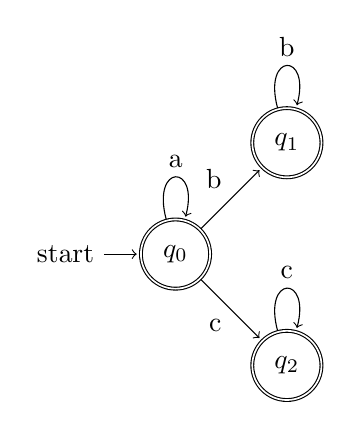
\begin{tikzpicture}[shorten >=1pt,node distance=2cm,on grid,auto] 
   \node[state,initial,accepting] (q_0)   {$q_0$}; 
   \node[state,accepting] (q_1) [above right=of q_0] {$q_1$}; 
   \node[state,accepting] (q_2) [below right=of q_0] {$q_2$};
    \path[->]
    (q_0) edge  node {b} (q_1)
          edge  node [swap] {c} (q_2)
          edge  [loop above] node {a} ()
    (q_1) edge [loop above] node  {b} ()
    (q_2) edge [loop above] node  {c} ();
\end{tikzpicture}
\end{align*}

Пересечением этих языков является язык $L_3$:

\begin{align*}
L_1 \cap L_2 = L_3 = \{ a^nb^n + a^nc^n\mid n \geqslant 0 \}
\end{align*}

который, как мы знаем, не является $LL(k)$ ни для какого $k$ (см пример 8.4 конспекта 11 лекции).

Отсюда делаем вывод, что класс LL языков не замкнут относительно пересечения с регулярными языками.

\end{document}